\documentclass{bioinfo}

% For \addlinespace and \bottomrule
\usepackage{booktabs}

% Place the caption above the table
\usepackage{float}
\floatstyle{plaintop}
\restylefloat{table}

\copyrightyear{2014}
\pubyear{2014}
\application % applications note

\begin{document}
\firstpage{1}

\title[UniqTag]{
UniqTag: Content-derived unique and stable identifiers for gene annotation}
\author[Jackman \textit{et al.}]{
Shaun Jackman$^{1,2,*}$, Joerg Bohlmann$^{3,4}$ and \.{I}nan\c{c} Birol$^{1,5}$
\footnote{to whom correspondence should be addressed}
}

\address{
$^1$Genome Sciences Centre, British Columbia Cancer Agency, Vancouver, BC, Canada
\\$^2$Graduate Program in Bioinformatics, University of British Columbia, Vancouver, BC, Canada
\\$^3$Michael Smith Laboratories, University of British Columbia, Vancouver, BC, Canada
\\$^4$Department of Forest Sciences, University of British Columbia, Vancouver, BC, Canada
\\$^5$Department of Medical Genetics, University of British Columbia, Vancouver, BC, Canada
}

\history{Received on XXXXX; revised on XXXXX; accepted on XXXXX}

\editor{Associate Editor: XXXXXXX}

\maketitle

\begin{abstract}
\section{Summary}\label{summary}

UniqTag assigns unique identifiers to gene sequences, or other arbitrary
sequences of characters, that are derived from the \emph{k}-mer
composition of the sequence. Unlike serial numbers, these identifiers
are stable between different assemblies and annotations of the same
data.

\section{Availability and
implementation}\label{availability-and-implementation}

The implementation of UniqTag is available at

\texttt{https://github.com/sjackman/uniqtag}

Supplementary data and code to reproduce it is available at

\texttt{https://github.com/sjackman/uniqtag-paper}

\section{Contact}\label{contact}

Shaun Jackman \textless{}sjackman@bcgsc.ca\textgreater{}

Inanc Birol \textless{}ibirol@bcgsc.ca\textgreater{}

\end{abstract}\section{Introduction}\label{introduction}

The task of annotating the genes of a genome sequence often follows
genome sequence assembly. These annotated genes are assigned unique
identifiers by which they can be referenced. Assembly and annotation is
often an iterative process, by refining the method or by the addition of
more sequencing data. These gene identifiers would ideally be stable
from one assembly and annotation to the next. Serial numbers are used
for identifiers of genes annotated by software such as MAKER
(\href{http://dx.doi.org/10.1104/pp.113.230144}{Campbell, 2014}), which,
although certainly unique, are not stable between assemblies. A single
change in the assembly can result in a total renumbering of the
annotated genes.

One solution to stabilize identifiers is to assign them based on the
content of the gene sequence. A cryptographic hash function such as SHA
(Secure Hash Algorithm)
(\href{http://www.nist.gov/manuscript-publication-search.cfm?pub_id=910977}{Dang,
2012}) derives a message digest from the sequence, such that two
sequences with the same content will have the same message digest, and
two sequences that differ will have different message digests. If a
cryptographic hash were used to identify a gene, the same gene in two
assemblies with identical content would be assigned identical
identifiers, but by design a slight change in the sequence, such as a
single-character substitution, would result in a completely different
digest and unique identifier.

A cryptographic hash function is designed so that small changes in the
message, even a single bit change, results in large changes to the
message digest: half of the bits of the digest are expected to flip,
called the avalanche effect
(\href{http://www.scientificamerican.com/article/cryptography-and-computer-privacy/}{Feistel,
1973}). Locality-sensitive hashing in contrast aims to assign items that
are similar to the same hash bucket. A hash function that, after a small
perturbation of the sequence, assigns an identical identifier to the
sequence is desirable for identifying the genes of a genome sequence
assembly project. One such locality-sensitive hash function, MinHash,
was employed in identifying web pages with similar content
(\href{http://dx.doi.org/10.1109/SEQUEN.1997.666900}{Broder, 1997}).
UniqTag implements MinHash, where the set of elements of an item is the
\emph{k}-mer composition of the sequence, the hash function is the
identity function and the minimal element is the lexicographically
minimal sequence, to assign stable identifiers to genes. These
identifiers are intended for systematic identification, unique within an
assembly, rather than as a biological name, which is typically assigned
based on biological function or homology to orthologous genes.

\section{Description}\label{description}

When iterating over multiple assemblies of the same data, it is rather
inconvenient when gene identifiers change from one assembly to the next.
UniqTag attempts to address this common challenge. By identifying the
gene by a feature of its content rather than an arbitrary serial number,
the gene identifier is stable between assemblies.

A UniqTag will change due to a difference in the locus of the UniqTag
itself, the creation of a least-frequent \emph{k}-mer that is
lexicographically smaller than the previous UniqTag, or the creation of
a \emph{k}-mer elsewhere resulting in the UniqTag no longer being a
least-frequent \emph{k}-mer. Concatenating two gene models results in a
gene whose UniqTag is the minimum of the two previous UniqTags, unless
one of the k-mer at the junction of the two sequences is
lexicographically smaller. Similarly when a gene model is split in two,
one gene is assigned a new UniqTag and the other retains the previous
UniqTag, unless the previous UniqTag spanned the junction.

A UniqTag can be generated from the nucleotide sequence of a gene. Using
instead the translated amino acid sequence of a protein-coding gene
sequence results in a UniqTag that is stable across synonymous changes
to the coding sequence as well as to changes in the untranslated regions
and introns of the gene. Since the amino acid alphabet is larger than
the nucleotide alphabet, fewer characters are required for a
\emph{k}-mer to be likely unique, resulting in an aesthetically pleasing
shorter identifier.

Two gene models with identical sequence would be assigned the same
UniqTag. It is possible that two genes that have no unique \emph{k}-mer
and similar \emph{k}-mer composition are assigned the same UniqTag.
Genes that have the same UniqTag are distinguished by adding a numerical
suffix to the UniqTag.

\subsection{Algorithm}\label{algorithm}

The UniqTag $u_k(s, S)$, a substring of the string \emph{s} with length
\emph{k} from the set of strings \emph{S}, is defined as follows.

$\Sigma$ is an alphabet. $\Sigma^k$ is the set of all strings over
$\Sigma$ of length \emph{k}. \emph{s} and \emph{t} are strings over
$\Sigma$. $C(s)$ is the set of all substrings of \emph{s}. A
\emph{k}-mer of \emph{s} is a substring of \emph{s} with length
\emph{k}. $C_k(s)$ is the set of all \emph{k}-mers of \emph{s}.

\[
C_k(s) = C(s) \cap \Sigma^k
\]

\emph{S} is a set of strings over $\Sigma$. $f(s, S)$ is the frequency
of \emph{s} in \emph{S}, defined as the number of strings in \emph{S}
that contain \emph{s} as a substring.

\[
f(s, S) = \left\vert \{ t \mid s \in C(t) \wedge t \in S \} \right\vert
\]

$\min S$ is the lexicographically minimal string of \emph{S}.
$u_k(s, S)$ is the UniqTag, the lexicographically minimal \emph{k}-mer
of those \emph{k}-mers of \emph{s} that are least frequent in \emph{S}.

\[
u_k(s, S) = \min \mathop{\arg\,\min}\limits_{t \in C_k(s)} f(t, S)
\]

\section{Results}\label{results}

UniqTag was used to assign nine-peptide identifiers to the first peptide
sequence, that with the smallest ENSP number, of each gene of the
Ensembl human genome. This analysis was repeated for nine builds of the
Ensembl human genome
(\href{http://dx.doi.org/10.1093/nar/gkt1196}{Flicek, 2014}) spanning
seven years and two major genome assemblies, NCBI36 up to build 54 and
GRCh37 afterward. The number of common UniqTag identifers between older
builds, from build 40 to build 74, and the current build 75 is shown in
Figure~1. Also shown is the number of common gene and protein
identifiers (ENSG and ENSP accession numbers) and the number of
identical peptides sequences between builds. Although less stable than
the gene ID, the UniqTag is more stable than the protein ID and the
peptide sequence. Whereas the gene and protein identifiers can, with
effort, be lifted over from older builds to the newest build, the
UniqTag identifier can be generated without any knowledge of previous
assemblies, making it a much simpler operation. The number of identical
peptide sequences between builds shows the performance that would be
expected of using a message digest, such as SHA-1, of the peptide
sequence as the identifier. Supplementary figure~S1 shows that the
UniqTag identifiers are quite stable for values of \emph{k}, the size of
the UniqTag identifier, between 8 and 50 peptides.

\begin{figure}[htbp]
\centering
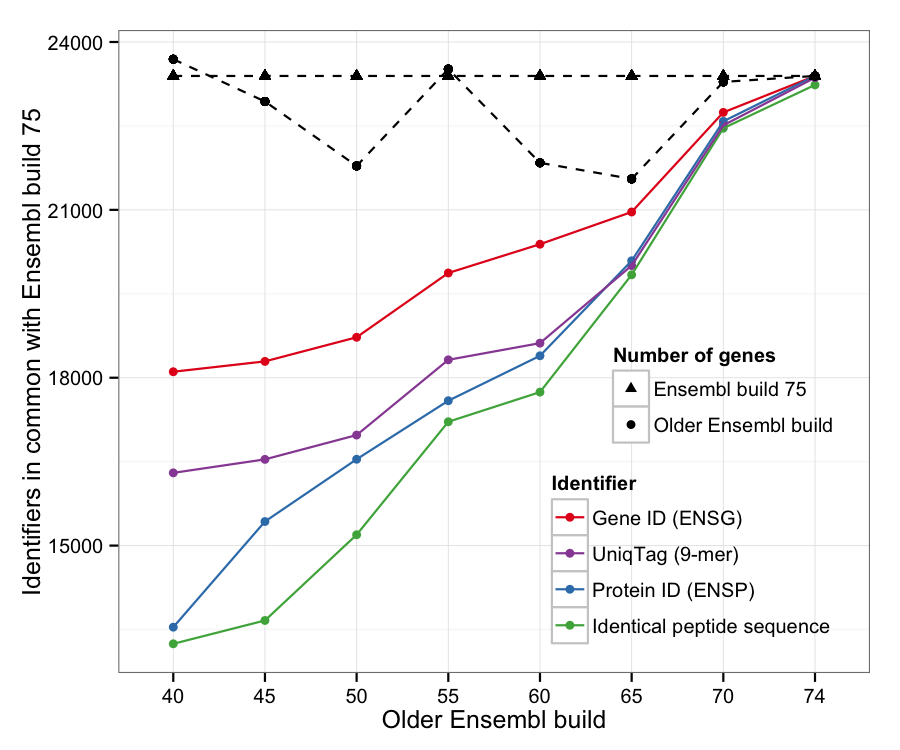
\includegraphics{ensembl.png}
\caption{The number of common UniqTag identifers between older builds of
the Ensembl human genome and the current build 75, the number of common
gene and protein identifiers, and the number of identical peptide
sequences between builds.}
\end{figure}

\section*{Acknowledgements}\label{acknowledgements}
\addcontentsline{toc}{section}{Acknowledgements}

The author thanks Nathaniel Street for his enthusiastic feedback, the
SMarTForests project and the organizers of the 2014 Conifer Genome
Summit that made our conversation possible.

\emph{Funding}: This work was supported by the Natural Sciences and
Engineering Research Council of Canada, Genome British Columbia, Genome
Alberta, Genome Quebec and Genome Canada.

\section*{References}\label{references}
\addcontentsline{toc}{section}{References}

\href{http://dx.doi.org/10.1109/SEQUEN.1997.666900}{Broder, A. Z.
(1997)} On the resemblance and containment of documents.
\emph{Compression and Complexity of Sequences}, 1997 Proceedings,
21-29.\\\href{http://dx.doi.org/10.1104/pp.113.230144}{Campbell, M. S.
\emph{et al.} (2014)} MAKER-P: a tool-kit for the rapid creation,
management, and quality control of plant genome annotations. \emph{Plant
Physiology}, 164(2),
513-524.\\\href{http://www.nist.gov/manuscript-publication-search.cfm?pub_id=910977}{Dang,
Q. H. (2012)} Secure Hash Standard (SHS). \emph{NIST FIPS}, 180(4),
1-35.\\\href{http://www.scientificamerican.com/article/cryptography-and-computer-privacy/}{Feistel,
H. (1973)} Cryptography and Computer Privacy. \emph{Scientific
American}, 228(5).\\\href{http://dx.doi.org/10.1093/nar/gkt1196}{Flicek,
P. \emph{et al.} (2014)} Ensembl 2014. \emph{Nucleic Acids Research},
42(D1), D749-D755.
\end{document}
